\documentclass[]{auvsi_doc}
\setkeys{auvsi_doc.cls}{
	AUVSITitle={Unmanned Ground Vehicle Requirements Matrix},
	AUVSIRevision=1.1,
	AUVSIDescription={Initial Draft},
	AUVSIAuthor={Kameron Eves},
	AUVSIChecker={?},
	AUVSILogoPath={./figs/logo.pdf},
	AUVSIDocID={RM-002}
}

% include extra packages, if needed
\usepackage[skip=-50pt]{caption}

% Remove Heading Numbers
\setcounter{secnumdepth}{0}

% Remove Heading Numbers
\setcounter{secnumdepth}{0}

\begin{document}
\begin{AUVSITitlePage}
\begin{artifacttable}
	\entry{RM-001, 0.1, 10-23-2018, Initial requirements,Jacob Willis, Brady Moon}
	\entry{RM-001, 1.1, 10-26-2018, Better performance measures,Jacob Willis, Kameron Eves}
	\entry{RM-001, 1.2, 10-26-2018, Edits after design review,Brady Moon \& John Akagi, Kameron Eves}
    \entry{RM-001, 2.0, 02-20-2019, Added measured values,Derek Knowles, Brandon McBride}
\end{artifacttable}
\end{AUVSITitlePage}
% document contents
%\begin{figure}
	\begin{center}
	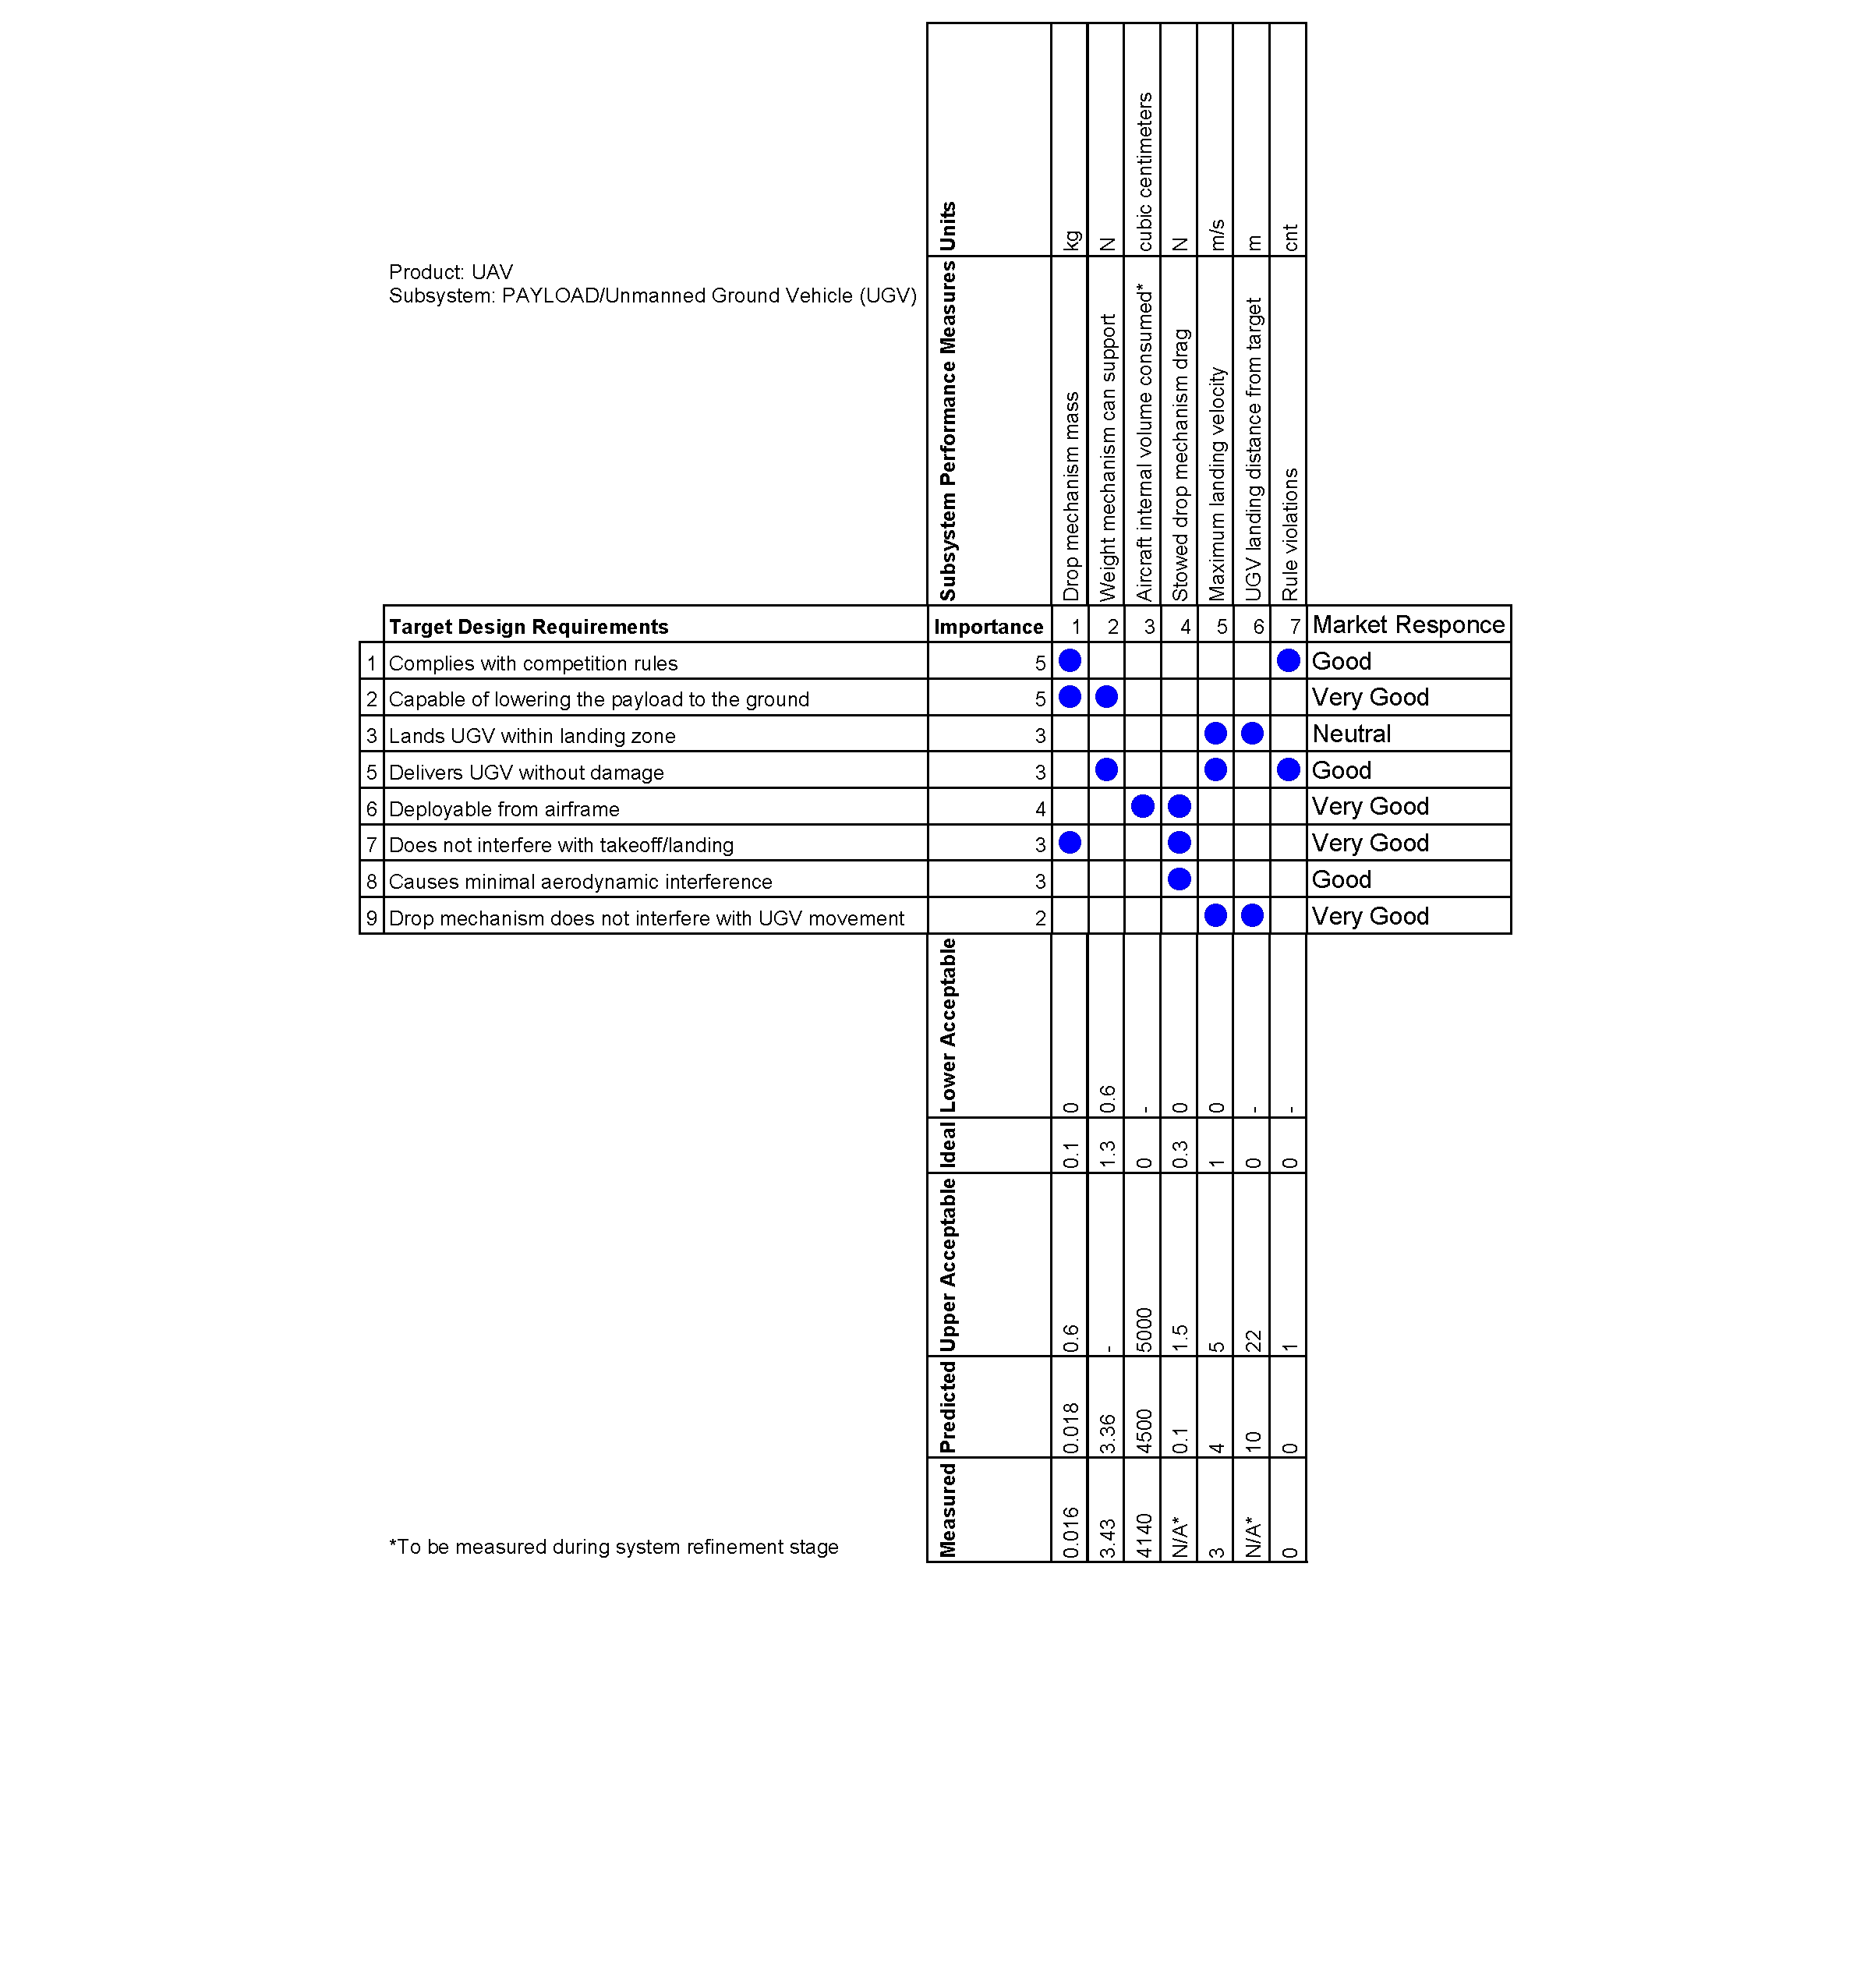
\includegraphics[width=0.95\textwidth]{./figs/RequirementsMatrix.pdf}
	\captionof{figure}{Requirements matrix for the subsystem which will deliver the UGV to the ground.}
	\label{fig:reqMat}
	\end{center}
%\end{figure}

\end{document}
